\section{Model pętli korowo-wzgórzowej Traub at al.}
Większość wyników powstała w oparciu o model pętli korowo wzgórzowej \cite{Traub2005}. Obejmuje on kolumnę korową wraz z wejściem ze wzgórza. Cały model zawiera 3560 wieloprzedziałowych komórek z 14 populacji z czego 12 w korze. Kolumna korowa składa się z 4 warstw odpowiadającym rzeczywistym warstwom:
\begin{itemize}
\item połączonym warstwom drugiej i trzeciej
\item warstwie czwartej
\item warstwie piątej
\item wastwie szóstej
\end{itemize}
Więcej szczegółów w tabeli \ref{tab:pop}. Morfologia komórek zostala pokazana na \ref{tarub_org}. Warto zuważyć, że rozmieszczenie dendrytów w przestrzeni nie ma znaczenia dla symulacji aktywności sieci neuronalnej (ale ma przy wyliczniu zewnątrzkomókowego potencjłu polowego) i w oryginalnej wersji dendryty umieszczone są w dwuwymiarowej przestrzeni \ref{tarub_org}.

\begin{table}[h!]
%  \begin{tabular}{|l|p{8.5cm}|p{2.6cm}|p{2cm}|}
  \begin{tabular}{|p{0.15\textwidth}|p{0.45\textwidth}|p{0.12\textwidth}|p{0.12\textwidth}|p{0.12\textwidth}|}
    \hline
    Położenie & Populacja & Skrócona nazwa & Ilość przedziałów & Ilość komórek w populacji\\
    \hline
    warstwa 2/3 & piramidalne o regularnej aktywności (pyramidal regular spiking) & pyrRS & 74 & 1000 \\
    \hline
    warstwa 2/3 & piramidalne o szybkich rytmicznych paczkach wyładowań (pyramidal fast rythmic bursting) & pyrFRB & 74  & 50 \\
    \hline
    warstwa 2/3 & interneurony warstwy powierzchniowej koszykowe (superficial interneurons basket) & bask & 50 & 90 \\
    \hline
    warstwa 2/3 & interneurony warstwy powierzchniowej axo-axonalne (superficial interneurons axoaxonic) & axax & 50 & 90 \\
    \hline
    warstwa 2/3 & interneurony warstwy powierzchniowej z niskim progiem (superficial interneurons low threshold spiking) & LTS & 50 & 90 \\
    \hline
    warstwa 4 & gwiaździste kolczaste (spiny stellate) & ss & 59 & 240 \\
    \hline
    warstwa 5 & piramidalne krzaczesta z samowyładującymi się (pyramidal tufted intrinsic bursting) & tuftIB & 61 & 800 \\
    \hline
    warstwa 5 &  piramidalne krzaczaste o regularnej aktywności (pyramidal tufted regular spiking) & tuftRS & 61 & 200\\
    \hline
    warstwa 5/6 & interneurony warstwy głębokiej koszykowe (deep interneurons basket) & deep bask & 59 & 100 \\
    \hline
    warstwa 5/6 & interneurony warstwy głębokiej axo-axonalne (deep interneurons axoaxonic) & deep axax & 59 & 100 \\
    \hline
    warstwa 5/6 & interneurony warstwy głębokiej o niskim progu aktywności (deep interneurons low threshold spiking) & deep LTS & 59 & 100 \\
    \hline
    warstwa  6 & piramidalne niekrzaczaste (pyramidal nontufted regular spiking) & nontuftRS & 59 & 500\\
    \hline
    Thalamus & thalamocortical relay & TCR & 139 & 100 \\
    \hline
    Thalamus & nucleus reticularis & nRT & 59 & 100 \\
    \hline
    Total & & & 3560 \\
    \hline
  \end{tabular}
  \caption{Rodzaje komórek występujące w modelu, nazwy przypisane im w oryginalnym artykule \cite{Traub2005}, ilość przedziałów, wielkość populacji
w pełnym modelu. W niektórych symulacjach zostało użyte tylko 10$\%$ komórek (10 $\%$ komórek z każdej populacji)}.
  \label{tab:pop}
\end{table}

\begin{figure}
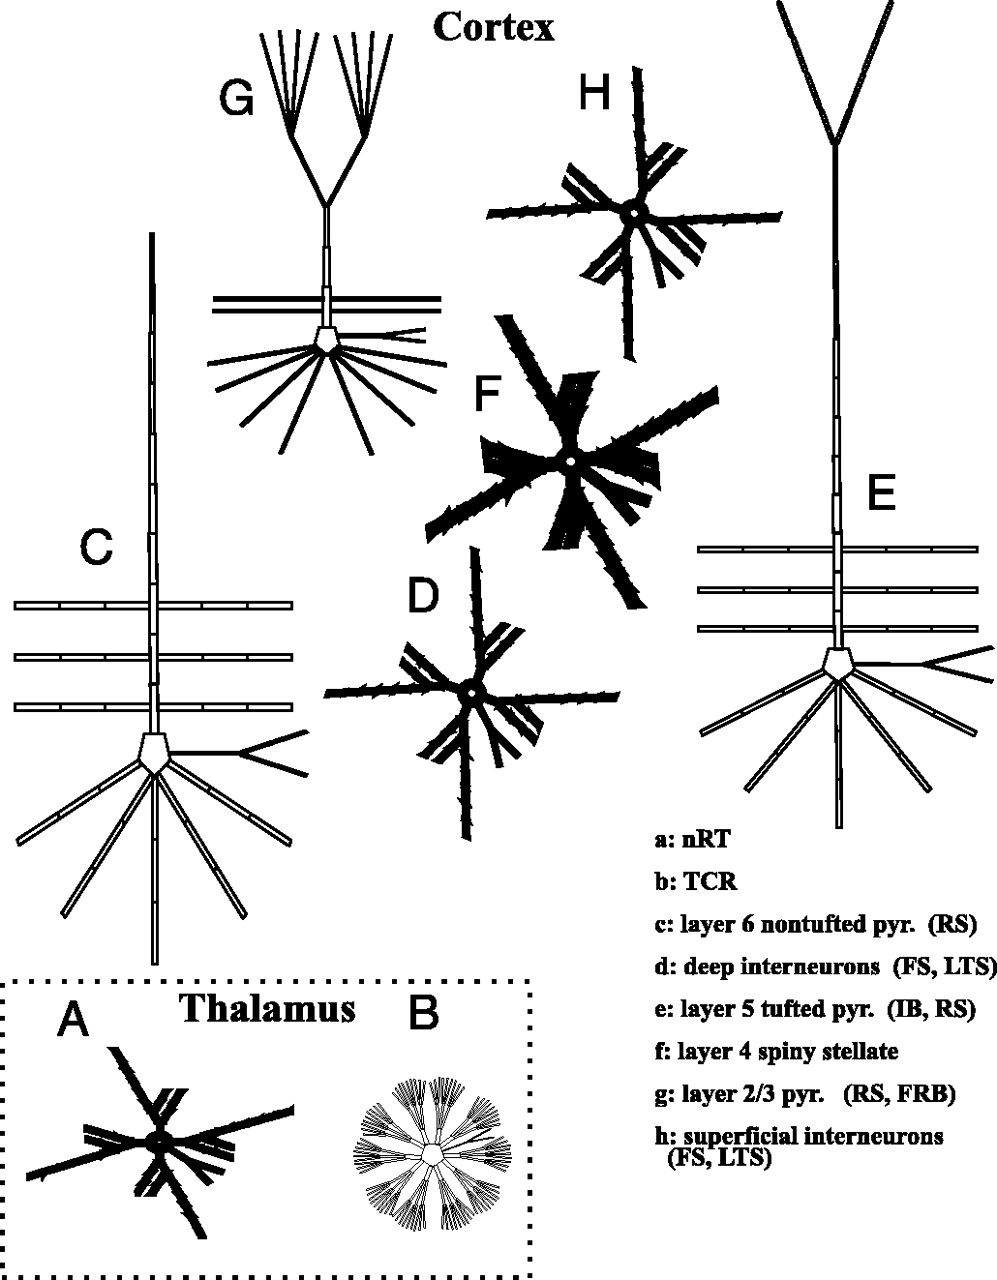
\includegraphics[width=0.5\textwidth]{../ryciny/F1.jpg} 
\label{tarub_org}
\caption{Reprodukcja z \cite{Traub2005} fig. 1}
\end{figure}

Oryginalny model powstał w Fortranie (ModelDB Accession:45539), w pracy korzystalismy z wersji przetłumaczonej na Neurona (ModelDB Accession: 82894). Informacje na temat rozmieszczenia drzew dendrytycznych w trójwymiarowej przestrzeni zaczerpnęliśmy z wersji w NeuroML (ModelDB Accession: 127353).